\documentclass[tikz,border=10pt]{standalone}

\usetikzlibrary{arrows.meta, positioning}

\begin{document}
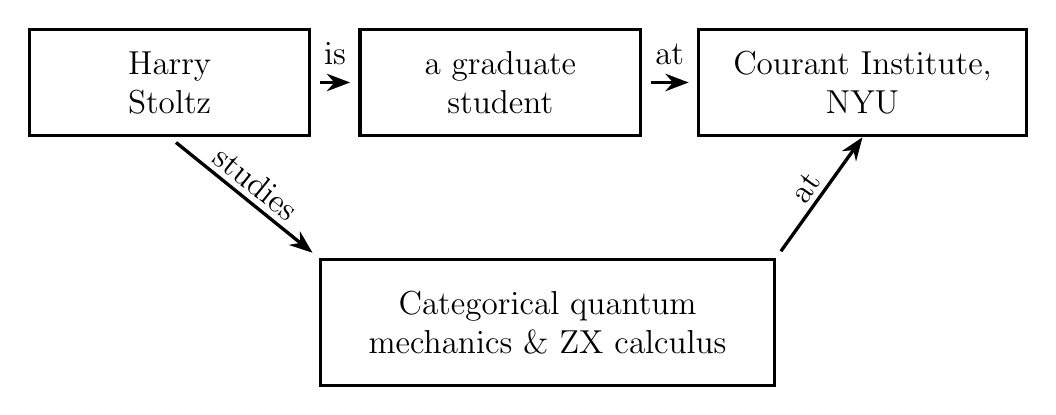
\begin{tikzpicture}[
  >=Stealth,
  olog box/.style={
    draw,
    very thick,
    align=center,
    text width=3.0cm,
    minimum height=1.35cm,
    inner sep=8pt,
    font=\large
  },
  olog arrow/.style={
    ->,
    very thick,
    shorten >=3pt,
    shorten <=3pt
  },
  label/.style={
    inner sep=2pt,
    font=\large
  }
]

\node[olog box] (harry) at (0, 1.7) {Harry\\Stoltz};
\node[olog box] (student) at (4.2, 1.7) {a graduate\\student};
\node[olog box, text width=3.6cm] (courant) at (8.8, 1.7) {Courant Institute,\\NYU};
\node[olog box, text width=5.2cm, minimum height=1.6cm] (research) at (4.8, -1.35)
  {Categorical quantum\\mechanics \& ZX calculus};

\draw[olog arrow] (harry) -- node[label, above=4pt] {is} (student);
\draw[olog arrow] (student) -- node[label, above=4pt] {at} (courant);
\draw[olog arrow] (harry.south) -- node[label, above, sloped] {studies} (research.north west);
\draw[olog arrow, shorten >=0pt] (research.north east) -- node[label, above, sloped] {at} (courant.south);

\end{tikzpicture}
\end{document}
